\begin{problem}{Skemmtilegar Setningar}{Inn}{Út}{~}{~}

	\begin{wrapfigure}{r}{0.43\textwidth}
		\vspace{-25pt}
		\begin{center}
			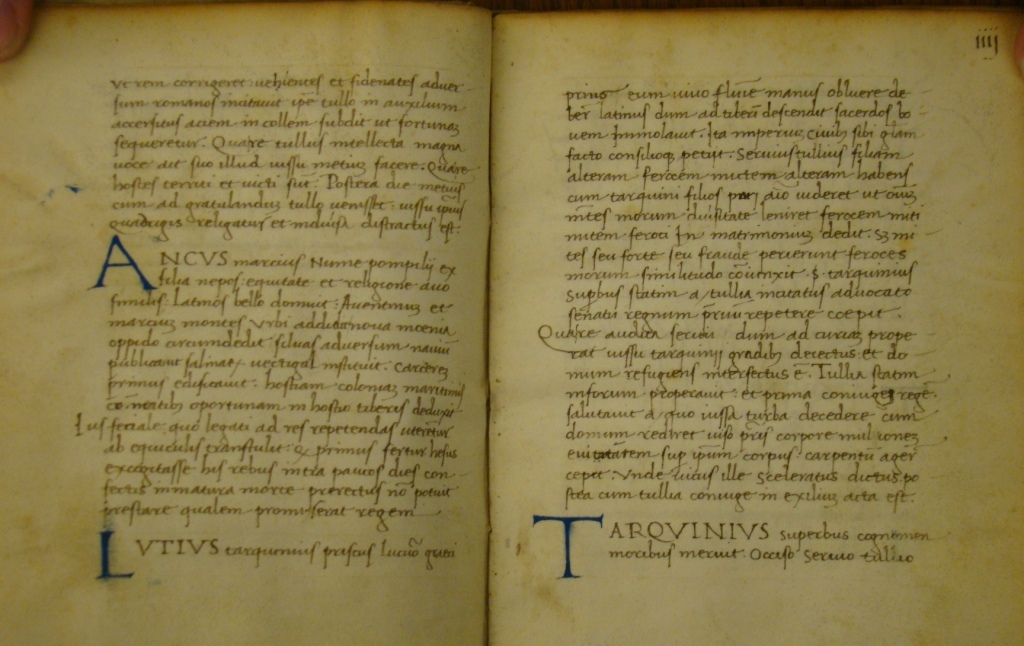
\includegraphics[scale=0.2]{../SkemmtilegarSetningar/book.jpg}
		\end{center}
		\vspace{-30pt}
	\end{wrapfigure}

	Setning samanstendur af orðum, aðskildum með bili, þar sem hvert orð er röð af bókstöfum. Setning getur svo endað á táknum eins og punkti, spurningamerki, eða upphrópunarmerki. Við skulum kalla setningu \textit{skemmtilega} ef að fyrir hvert par af samliggjandi orðum gildir að síðasti stafurinn í fyrra orðinu er sá sami og fyrsti stafurinn í seinna orðinu. Þá er til dæmis setningin "`Ýmir rúllaði inní ísbúðina!"' skemmtileg, en við sjáum að síðasti stafurinn í "`Ýmir"' er sá sami og fyrsti stafurinn í "`rúllaði"', og það sama gildir fyrir "`rúllaði"' og "`inní"', og "`inní"' og "`ísbúðina"'. Athuga skal að ekki er gerður greinarmunur á hástaf og lágstaf. Ef setning er ekki \textit{skemmtileg}, þá er hún auðvitað kölluð \textit{leiðinleg}.
	
	\Input

		Á fyrstu línu er heiltalan $1 \leq T \leq 100$, sem táknar fjölda prófunartilvika sem fylgja. Hvert prófunartilvik samanstendur af einni línu sem inniheldur eina setningu, þar sem setning er skilgreind að ofan.

	\Output

		Fyrir hvert prófunartilvik á að skrifa út eina línu sem inniheldur "`\texttt{Fun}"' ef setningin er skemmtileg, en "`\texttt{Boring}"' ef setningin er leiðinleg.

	\Examples

		\begin{example}
			\exmp{
6
Hvernig gengur?
Forritunarkeppnin er awesome.
Was she early?
Abba Abba abba.
Abba babba babb.
John needs sugar!
}{
Fun
Boring
Fun
Fun
Boring
Fun
}%
		\end{example}

\end{problem}